\documentclass[aspectratio=169, table, 12pt]{beamer}

\usepackage{colortbl}
\usepackage{xcolor}
\usepackage{listings}
\usepackage{tabularx}
\usepackage{tikz}
\usetikzlibrary{arrows.meta, positioning, calc, fit, shapes.geometric}

\makeatletter
\def\input@path{{../theme/}}
\makeatother
\graphicspath{{../theme/}{../../figures/}}
\usetheme{Pradita}

\definecolor{praditagreen}{RGB}{37, 113, 71}

% Tema membuat garis tabel berwarna putih. Dikembalikan agar tabel terbaca.
\arrayrulecolor{black}
\setlength{\arrayrulewidth}{0.5pt}

% Kolom X rata kiri, dipakai pada tabel dengan kolom X yang sempit, agar
% spasi antarkata tidak meregang.
\newcolumntype{Y}{>{\raggedright\arraybackslash}X}

\lstdefinelanguage{bash}{
  keywords={},
  basicstyle=\ttfamily\scriptsize,
  ndkeywords={cd, coverage, curl, diff, docker, echo, npm, npx, python,
              python3, pytest, source},
  ndkeywordstyle=\color{purple}\bfseries,
  sensitive=true,
  commentstyle=\color{gray},
  numbers=none,
  breaklines=true,
  frame=lines,
  backgroundcolor=\color{lightgray!10},
  tabsize=2,
  comment=[l]{\#},
  showstringspaces=false
}

\lstdefinelanguage{TypeScript}{
  keywords={const, let, function, return, async, await, try, catch, throw,
            new, if, interface, void, export, import, from, type},
  ndkeywords={Promise, number, string, boolean, test, expect, Page, await},
  basicstyle=\ttfamily\scriptsize,
  keywordstyle=\color{blue}\bfseries,
  ndkeywordstyle=\color{purple}\bfseries,
  sensitive=true,
  commentstyle=\color{gray}\itshape,
  stringstyle=\color{red},
  numbers=none,
  breaklines=true,
  frame=lines,
  backgroundcolor=\color{lightgray!10},
  tabsize=2,
  comment=[l]{//},
  morestring=[b]",
  showstringspaces=false
}

% Gaya Python disamakan dengan naskah bab, tanpa nomor baris.
\lstdefinestyle{PythonStyle}{
  language=Python,
  basicstyle=\ttfamily\scriptsize,
  morekeywords={with, as, yield, async, await, match, case},
  keywordstyle=\color{blue}\bfseries,
  emph={pytest, psycopg, Mock, given, strategies},
  emphstyle=\color{purple}\bfseries,
  commentstyle=\color{gray}\itshape,
  stringstyle=\color{red},
  numbers=none,
  breaklines=true,
  frame=lines,
  backgroundcolor=\color{lightgray!10},
  tabsize=2,
  showstringspaces=false
}

% File mutu dan kontrak ditampilkan apa adanya, sehingga butuh gaya JSON.
\lstdefinelanguage{json}{
  basicstyle=\ttfamily\scriptsize,
  stringstyle=\color{red},
  commentstyle=\color{gray},
  numbers=none,
  breaklines=true,
  frame=lines,
  backgroundcolor=\color{lightgray!10},
  tabsize=2,
  showstringspaces=false,
  morestring=[b]"
}

\title{\Huge Arsitektur\\ \vspace{10pt} Web Modern}
\subtitle{IF140303 - Pengembangan Aplikasi Web}
\author{\textbf{Alfa Yohannis}}

\begin{document}

\frame{\titlepage}

\begin{frame}[fragile]
  \frametitle{Isi Pertemuan}
  \vspace{14pt}
  \begin{columns}[t]
    \column{0.5\textwidth}
    {\small\tableofcontents[sections={1-7}]}

    \column{0.5\textwidth}
    {\small\tableofcontents[sections={8-14}]}
  \end{columns}
\end{frame}

\begin{frame}{\hfill}
  \centering
  \Huge{\textbf{Di mana sebaiknya\\halaman dirakit?}}
\end{frame}

\section{Tujuan dan Kerangka Bahasan}

\begin{frame}{\hfill}
  \centering
  \Huge{\textbf{Tujuan dan Kerangka Bahasan}}
\end{frame}

\begin{frame}{{\Large Tujuan Pembelajaran}}
  \vspace{10pt}
  \begin{itemize}
    \item Membedakan tempat HTML dirakit pada SPA, SSR, SSG, ISR, dan
          \textit{islands}, lalu menyebut akibatnya pada jumlah permintaan
          dan waktu sampai isi tampil.
    \item Mengukur kelima varian pada halaman yang sama, lalu membaca
          selisihnya dari byte yang tiba dan jumlah permintaan.
    \item Memilih satu arsitektur untuk kebutuhan tertentu, lalu
          mempertanggungjawabkannya sebagai catatan keputusan.
  \end{itemize}
\end{frame}

\begin{frame}{{\Large Yang Dibandingkan Bab Ini}}
  \vspace{12pt}
  \begin{itemize}
    \item Bab 2 sampai 7 memperbaiki satu aplikasi dari dalam. Bab ini mundur
          satu langkah: di mana halaman sebaiknya dirakit.
    \item Perbedaannya sering dibahas sebagai selera, padahal sebagian besar
          dapat dihitung.
  \end{itemize}
  \vspace{8pt}
  {\small Demonya sengaja kecil: satu file Python, tanpa basis data dan tanpa
  container, karena yang dibandingkan tempat perakitannya, bukan cara datanya
  diambil.}
\end{frame}

\section{Dari Tradisional ke SPA}

\begin{frame}{\hfill}
  \centering
  \Huge{\textbf{Dari Tradisional\\ke Single-Page Application}}
\end{frame}

\begin{frame}{{\Large Dua Pembagian Tugas}}
  \vspace{12pt}
  \begin{itemize}
    \item \textbf{SSR}: server merakit HTML pada tiap permintaan, browser
          menerima halaman yang sudah jadi.
    \item \textbf{SPA}: server mengirim kerangka hampir kosong beserta
          JavaScript, lalu browser yang meminta data dan menggambar isinya.
  \end{itemize}
  \vspace{8pt}
  {\small Analoginya memesan makanan. SSR mengantar piring yang sudah terisi.
  SPA mengantar piring kosong beserta bahan dan kompornya, lalu memasaknya di
  meja pemesan.}
\end{frame}

\begin{frame}{{\Large SSR lawan SPA, Diukur}}
  \vspace{6pt}
  \centering
  {\footnotesize
  \begin{tabularx}{\textwidth}{Yrr}
    \hline
    \textbf{Ukuran} & \textbf{SSR} & \textbf{SPA} \\
    \hline
    Byte HTML yang pertama tiba & 511 & 229 \\
    \hline
    Byte seluruhnya sampai isi tampil & 511 & 1.551 \\
    \hline
    Permintaan sampai isi tampil & 1 & 3 \\
    \hline
    Isi katalog ada di HTML pertama & ya & tidak \\
    \hline
  \end{tabularx}}

  \vspace{8pt}
  {\small Baris terakhir yang paling menentukan. HTML varian SPA memang
  paling kecil, tetapi di dalamnya tidak ada satu judul buku pun.}
\end{frame}

\section{SSR, SSG, dan ISR}

\begin{frame}{\hfill}
  \centering
  \Huge{\textbf{SSR, SSG, dan ISR}}
\end{frame}

\begin{frame}{{\Large Bedanya Hanya Kapan Dirakit}}
  \vspace{10pt}
  \centering
  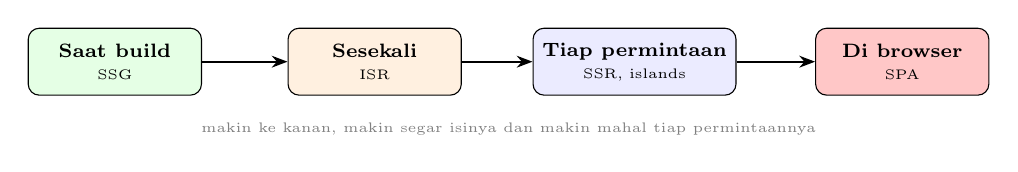
\begin{tikzpicture}[
    font=\scriptsize,
    kotak/.style={draw, rounded corners, minimum height=0.85cm,
                  minimum width=2.2cm, align=center, font=\scriptsize\bfseries},
    panah/.style={-{Stealth[length=2mm]}, thick}
  ]
    \node[kotak, fill=green!10] (build) at (0,0) {Saat build\\{\tiny\mdseries SSG}};
    \node[kotak, fill=orange!12] (sesekali) at (3.3,0) {Sesekali\\{\tiny\mdseries ISR}};
    \node[kotak, fill=blue!8] (tiap) at (6.6,0) {Tiap permintaan\\{\tiny\mdseries SSR, islands}};
    \node[kotak, fill=red!22] (browser) at (10.0,0) {Di browser\\{\tiny\mdseries SPA}};

    \draw[panah] (build) -- (sesekali);
    \draw[panah] (sesekali) -- (tiap);
    \draw[panah] (tiap) -- (browser);
    \node[font=\tiny, gray, anchor=north] at (5.0,-0.65)
      {makin ke kanan, makin segar isinya dan makin mahal tiap permintaannya};
  \end{tikzpicture}

  \vspace{10pt}
  {\small SSG merakit sekali saat \textit{build}, ISR merakit ulang sesekali,
  SSR merakit pada tiap permintaan.}
\end{frame}

\begin{frame}{{\Large Lima Varian, Halaman yang Sama}}
  \vspace{6pt}
  \centering
  {\footnotesize
  \begin{tabularx}{\textwidth}{lrrlrr}
    \hline
    \textbf{Varian} & \textbf{HTML} & \textbf{Total} & \textbf{Isi di HTML} & \textbf{Minta} & \textbf{Total ms} \\
    \hline
    SSG & 511 B & 511 B & ya & 1 & 1,9 \\
    \hline
    ISR & 511 B & 511 B & ya & 1 & 52,9 \\
    \hline
    SSR & 511 B & 511 B & ya & 1 & 51,8 \\
    \hline
    Islands & 625 B & 1.322 B & ya & 2 & 3,1 \\
    \hline
    SPA & 229 B & 1.551 B & tidak & 3 & 1,7 \\
    \hline
  \end{tabularx}}

  \vspace{6pt}
  {\footnotesize Perakitan halaman diberi jeda 50 milidetik, mewakili halaman
  yang isinya mahal dihitung. Baris ISR mahal karena pengukurannya jatuh pada
  permintaan pertama sesudah kedaluwarsa. Baris SPA terlihat singkat karena
  yang diukur hanya waktu jaringannya.}
\end{frame}

\begin{frame}[fragile]{{\Large Inti ISR dalam Delapan Baris}}
  \vspace{2pt}
\begin{lstlisting}[style=PythonStyle]
def baca_atau_rakit_isr():
  """Membaca file ISR, dan merakitnya ulang bila umurnya sudah lewat.

  Inilah inti Incremental Static Regeneration: pengunjung tetap dilayani
  file yang sudah jadi, sedangkan perakitan ulang hanya terjadi sesekali.
  """
  if FILE_ISR.exists():
    umur = time.time() - FILE_ISR.stat().st_mtime
    if umur < UMUR_ISR_DETIK:
      return FILE_ISR.read_bytes(), "file lama dipakai"
  FILE_ISR.write_text(rakit_halaman_katalog(), encoding="utf-8")
  return FILE_ISR.read_bytes(), "dirakit ulang"
\end{lstlisting}
\end{frame}

\begin{frame}{{\Large Daur ISR dalam Lima Permintaan}}
  \vspace{6pt}
  \centering
  {\footnotesize
  \begin{tabularx}{\textwidth}{rYr}
    \hline
    \textbf{Permintaan} & \textbf{Keterangan dari header \texttt{X-ISR}} & \textbf{Waktu} \\
    \hline
    1 & dirakit ulang & 53,5 ms \\
    \hline
    2 & file lama dipakai & 1,9 ms \\
    \hline
    3 & file lama dipakai & 0,7 ms \\
    \hline
    4 & dirakit ulang, sesudah jeda sebelas detik & 51,5 ms \\
    \hline
    5 & file lama dipakai & 1,0 ms \\
    \hline
  \end{tabularx}}

  \vspace{8pt}
  {\small Biaya perakitan tidak hilang, melainkan ditanggung satu pengunjung
  tiap satu periode. Sisanya dilayani secepat SSG.}
\end{frame}

\section{Islands Architecture}

\begin{frame}{\hfill}
  \centering
  \Huge{\textbf{Islands Architecture}}
\end{frame}

\begin{frame}{{\Large Hanya Bagian Kecil yang Dihidupkan}}
  \vspace{6pt}
  \centering
  {\footnotesize
  \begin{tabularx}{\textwidth}{Yrr}
    \hline
    \textbf{Ukuran} & \textbf{Islands} & \textbf{SPA} \\
    \hline
    Byte HTML yang pertama tiba & 625 & 229 \\
    \hline
    Byte JavaScript yang diunduh & 697 & 938 \\
    \hline
    Permintaan sampai isi tampil & 2 & 3 \\
    \hline
    Isi tetap tampil bila skripnya gagal & ya & tidak \\
    \hline
  \end{tabularx}}

  \vspace{8pt}
  {\small Pada demo ini pulaunya hanya satu, yaitu kotak penyaring judul.
  Daftar bukunya sudah tergambar dari HTML yang dikirim server.}
\end{frame}

\section{Server dan Client Component}

\begin{frame}{\hfill}
  \centering
  \Huge{\textbf{Server Component\\dan Client Component}}
\end{frame}

\begin{frame}{{\Large Pembagian Tugasnya}}
  \vspace{6pt}
  \centering
  {\footnotesize
  \begin{tabularx}{\textwidth}{lYY}
    \hline
    \textbf{Hal} & \textbf{Server component} & \textbf{Client component} \\
    \hline
    Tempat berjalan & Server & Browser \\
    \hline
    Ikut diunduh & Tidak & Ya \\
    \hline
    Boleh menyentuh basis data & Ya & Tidak \\
    \hline
    Boleh memakai \textit{state} & Tidak & Ya \\
    \hline
    Pantas untuk & Daftar, artikel, halaman detail & Tombol, formulir, penyaring \\
    \hline
  \end{tabularx}}

  \vspace{8pt}
  {\small Pembagian inilah yang membuat \textit{islands} dapat ditulis tanpa
  memisahkan dua proyek.}
\end{frame}

\section{Edge dan Origin}

\begin{frame}{\hfill}
  \centering
  \Huge{\textbf{Edge dan Origin}}
\end{frame}

\begin{frame}{{\Large Apa yang Pantas Pindah ke Edge}}
  \vspace{6pt}
  \centering
  {\footnotesize
  \begin{tabularx}{\textwidth}{Yl}
    \hline
    \textbf{Pekerjaan} & \textbf{Tempatnya} \\
    \hline
    Melayani file statis dan halaman hasil SSG & \textit{Edge} \\
    \hline
    Mengarahkan pengunjung menurut negara atau bahasa & \textit{Edge} \\
    \hline
    Memeriksa token sesi sebelum permintaan diteruskan & \textit{Edge} \\
    \hline
    Menulis pesanan dan memotong stok & \textit{Origin} \\
    \hline
    Menjalankan agregat yang menyentuh banyak tabel & \textit{Origin} \\
    \hline
  \end{tabularx}}

  \vspace{6pt}
  {\footnotesize Dua hal sering tertukar: menyimpan \textit{copy} di
  \textit{edge} memindahkan salinan, sedangkan menjalankan kode di
  \textit{edge} memindahkan perhitungan, dan di sana jarak ke basis data
  justru bertambah jauh.}
\end{frame}

\section{Monolith, Modular Monolith, dan BFF}

\begin{frame}{\hfill}
  \centering
  \Huge{\textbf{Monolith, Modular Monolith,\\dan BFF}}
\end{frame}

\begin{frame}{{\Large Tiga Cara Membagi Kode Sisi Server}}
  \vspace{10pt}
  \centering
  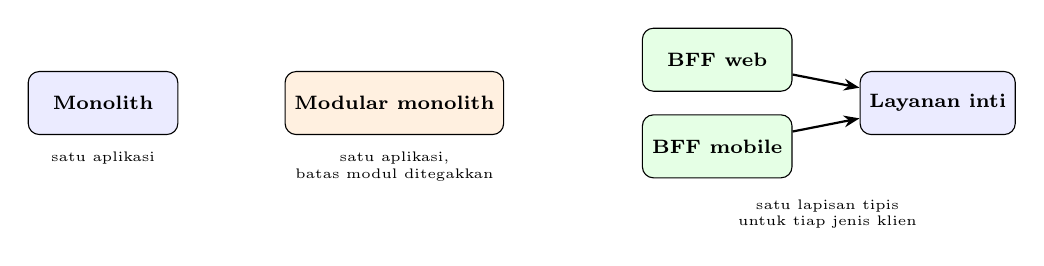
\begin{tikzpicture}[
    font=\scriptsize,
    kotak/.style={draw, rounded corners, minimum height=0.8cm,
                  minimum width=1.9cm, align=center, font=\scriptsize\bfseries},
    panah/.style={-{Stealth[length=2mm]}, thick}
  ]
    \node[kotak, fill=blue!8] (mono) at (0,0) {Monolith};
    \node[font=\tiny, anchor=north] at (0,-0.5) {satu aplikasi};

    \node[kotak, fill=orange!12, minimum width=2.7cm] (modular) at (3.7,0)
      {Modular monolith};
    \node[font=\tiny, anchor=north, align=center] at (3.7,-0.5)
      {satu aplikasi,\\batas modul ditegakkan};

    \node[kotak, fill=green!10] (bff1) at (7.8,0.55) {BFF web};
    \node[kotak, fill=green!10] (bff2) at (7.8,-0.55) {BFF mobile};
    \node[kotak, fill=blue!8] (inti) at (10.6,0) {Layanan inti};
    \draw[panah] (bff1) -- (inti);
    \draw[panah] (bff2) -- (inti);
    \node[font=\tiny, anchor=north, align=center] at (9.2,-1.1)
      {satu lapisan tipis\\untuk tiap jenis klien};
  \end{tikzpicture}

  \vspace{10pt}
  {\small Urutannya juga urutan yang disarankan ketika ragu: mulai dari
  \textit{monolith}, pecah ketika batasnya sudah kelihatan.}
\end{frame}

\section{Trade-off dan Catatan Keputusan}

\begin{frame}{\hfill}
  \centering
  \Huge{\textbf{Mempertanggungjawabkan\\Trade-off}}
\end{frame}

\begin{frame}{{\Large Catatan Keputusan Arsitektur}}
  \vspace{6pt}
  \centering
  {\footnotesize
  \begin{tabularx}{\textwidth}{lY}
    \hline
    \textbf{Bagian} & \textbf{Isinya} \\
    \hline
    Keputusan & Halaman katalog publik memakai ISR, umur sepuluh menit \\
    \hline
    Dipertimbangkan & SSR, SSG, dan ISR \\
    \hline
    Alasan & SSR menanggung 51,8 ms tiap permintaan, SSG terlalu kaku untuk isi yang berubah beberapa kali sehari \\
    \hline
    Konsekuensi & Satu pengunjung tiap periode menanggung 52,9 ms, isi dapat \textit{stale} sampai sepuluh menit \\
    \hline
    Yang membatalkan & Isi wajib segar seketika, atau perakitannya jauh lebih mahal \\
    \hline
  \end{tabularx}}

  \vspace{6pt}
  {\footnotesize Baris terakhir yang paling sering dilupakan: keputusan dapat
  ditinjau ulang dengan memeriksa syarat, bukan dengan mengulang perdebatan.}
\end{frame}

\section{Persiapan Latihan}

\begin{frame}{\hfill}
  \centering
  \Huge{\textbf{Persiapan Latihan}}
\end{frame}

\begin{frame}[fragile]{{\Large Satu Perintah Saja}}
  \vspace{2pt}
\begin{lstlisting}[language=bash]
cd sources/chapter08
python3 bangun-statis.py
python3 aplikasi.py &

# Keluarannya:
# Dibangun     : katalog-ssg.html
# Ukuran       : 511 byte
# Lama merakit : 0.3 ms
# Melayani di http://127.0.0.1:8040/ssr  (Ctrl+C untuk berhenti)
\end{lstlisting}
  \vspace{2pt}
  {\small Tanpa Docker dan tanpa Node.js. Seluruh pengukuran diarahkan ke
  aplikasi di komputer sendiri, dengan beban setara satu pengunjung.}
\end{frame}

\section{Latihan 1: Lima Varian}

\begin{frame}{\hfill}
  \centering
  \Huge{\textbf{Latihan 1\\Membandingkan Lima Varian}}
\end{frame}

\begin{frame}[fragile]{{\Large Langkah Kerja dan Perintahnya}}
  \vspace{2pt}
  {\footnotesize Jalankan alat ukurnya, buka kelima alamat di browser dengan
  JavaScript dimatikan, lalu lihat sumber halaman tiap varian.}
  \vspace{2pt}
\begin{lstlisting}[language=bash]
python3 ukur-varian.py

# Keluarannya:
#   Varian        HTML   Total  Isi di HTML  Minta  HTML ms  Total ms
#   ssg            511     511           ya      1      1.9       1.9
#   isr            511     511           ya      1     52.9      52.9
#   ssr            511     511           ya      1     51.8      51.8
#   islands        625    1322           ya      2      1.5       3.1
#   spa            229    1551        tidak      3      0.9       1.7
\end{lstlisting}
\end{frame}

\begin{frame}{{\Large Lembar Isian Latihan 1}}
  \vspace{6pt}
  \centering
  {\footnotesize
  \begin{tabularx}{\textwidth}{lrrlr}
    \hline
    \textbf{Varian} & \textbf{HTML} & \textbf{Total} & \textbf{Isi di HTML} & \textbf{Minta} \\
    \hline
    SSG & \dots & \dots & \dots & \dots \\
    \hline
    ISR & \dots & \dots & \dots & \dots \\
    \hline
    SSR & \dots & \dots & \dots & \dots \\
    \hline
    Islands & \dots & \dots & \dots & \dots \\
    \hline
    SPA & \dots & \dots & \dots & \dots \\
    \hline
  \end{tabularx}}

  \vspace{6pt}
  {\footnotesize Pertanyaan: mengapa HTML varian SPA paling kecil tetapi
  totalnya paling besar, mengapa alat ukur ini tidak menangkap seluruh biaya
  SPA, dan varian mana yang paling tahan terhadap skrip yang gagal dimuat?}
\end{frame}

\section{Latihan 2: Daur ISR}

\begin{frame}{\hfill}
  \centering
  \Huge{\textbf{Latihan 2\\Membaca Perilaku ISR}}
\end{frame}

\begin{frame}[fragile]{{\Large Mengamati Daurnya}}
  \vspace{2pt}
\begin{lstlisting}[language=bash]
curl -s -D - -o /dev/null -w "%{time_total}\n" http://127.0.0.1:8040/isr \
  | grep -iE "^(x-isr|[0-9])"

# Keluarannya:
# X-ISR: dirakit ulang
# 0.053519
\end{lstlisting}
  \vspace{4pt}
  {\small Minta tiga kali berurutan, tunggu sebelas detik, lalu minta dua
  kali lagi. Sesudah itu ubah \texttt{UMUR\_ISR\_DETIK} menjadi 60 dan ulangi
  pengamatannya.}
\end{frame}

\begin{frame}{{\Large Lembar Isian Latihan 2}}
  \vspace{6pt}
  \centering
  {\footnotesize
  \begin{tabularx}{\textwidth}{rYr}
    \hline
    \textbf{Permintaan} & \textbf{Keterangan \texttt{X-ISR}} & \textbf{Waktu} \\
    \hline
    1 & \dots & \dots \\
    \hline
    2 & \dots & \dots \\
    \hline
    3 & \dots & \dots \\
    \hline
    4, sesudah jeda sebelas detik & \dots & \dots \\
    \hline
    5 & \dots & \dots \\
    \hline
  \end{tabularx}}

  \vspace{6pt}
  {\footnotesize Pertanyaan: pengunjung mana yang menanggung biaya
  perakitan, dan apa yang berubah bila umurnya dinaikkan menjadi satu jam?}
\end{frame}

\section{Latihan 3: Menambah Pulau}

\begin{frame}{\hfill}
  \centering
  \Huge{\textbf{Latihan 3\\Memindahkan Satu Bagian\\Menjadi Pulau}}
\end{frame}

\begin{frame}[fragile]{{\Large Membandingkan Ukuran Skripnya}}
  \vspace{2pt}
\begin{lstlisting}[language=bash]
wc -c statis/pulau.js statis/spa.js

# Keluarannya:
#  697 statis/pulau.js
#  938 statis/spa.js
\end{lstlisting}
  \vspace{4pt}
  {\small Tambahkan satu pulau kedua pada halaman islands, misalnya tombol
  yang mengurutkan daftar menurut harga, lalu ukur ulang kedua varian.}
\end{frame}

\begin{frame}{{\Large Contoh Hasil dan Lembar Isian Latihan 3}}
  \vspace{4pt}
  \centering
  {\footnotesize
  \begin{tabularx}{\textwidth}{Yrr}
    \hline
    \textbf{Varian} & \textbf{Byte skrip} & \textbf{Byte total} \\
    \hline
    Islands, satu pulau & 697 & 1.322 \\
    \hline
    SPA & 938 & 1.551 \\
    \hline
  \end{tabularx}}

  \vspace{6pt}
  \centering
  {\footnotesize
  \begin{tabularx}{\textwidth}{Yrr}
    \hline
    \textbf{Varian} & \textbf{Byte skrip} & \textbf{Byte total} \\
    \hline
    Islands, satu pulau & \dots & \dots \\
    \hline
    Islands, dua pulau & \dots & \dots \\
    \hline
    SPA & \dots & \dots \\
    \hline
  \end{tabularx}}

  \vspace{4pt}
  {\footnotesize Pertanyaan: berapa byte yang bertambah tiap pulau baru, dan
  pada titik mana menambah pulau tidak lagi lebih murah daripada SPA?}
\end{frame}

\section{Latihan 4: Catatan Keputusan}

\begin{frame}{\hfill}
  \centering
  \Huge{\textbf{Latihan 4\\Menulis Catatan Keputusan}}
\end{frame}

\begin{frame}{{\Large Langkah Kerja}}
  \vspace{8pt}
  \begin{enumerate}
    \item Pilih satu kebutuhan nyata: katalog publik, rincian pesanan milik
          pengguna yang sudah masuk, atau papan kendali admin.
    \item Pilih tiga varian yang masuk akal bagi kebutuhan itu, lalu tulis
          angka pembandingnya dari Latihan 1.
    \item Tulis catatan keputusan berisi lima bagian: keputusan, yang
          dipertimbangkan, alasan beserta angkanya, konsekuensi, dan syarat
          yang membatalkannya.
  \end{enumerate}
  \vspace{8pt}
  {\small Hasilnya satu halaman saja. Yang dinilai bukan panjangnya,
  melainkan apakah angkanya dipakai dan konsekuensinya disebut.}
\end{frame}

\begin{frame}{{\Large Lembar Isian Latihan 4}}
  \vspace{6pt}
  \centering
  {\footnotesize
  \begin{tabularx}{\textwidth}{lY}
    \hline
    \textbf{Bagian} & \textbf{Isinya} \\
    \hline
    Kebutuhan yang dipilih & \dots \\
    \hline
    Keputusan & \dots \\
    \hline
    Dipertimbangkan & \dots \\
    \hline
    Alasan, beserta angkanya & \dots \\
    \hline
    Konsekuensi & \dots \\
    \hline
    Yang membatalkan & \dots \\
    \hline
  \end{tabularx}}

  \vspace{6pt}
  {\footnotesize Pertanyaan: angka mana yang paling menentukan pilihan Anda,
  dan keadaan apa yang akan membuat keputusan itu perlu ditinjau ulang?}
\end{frame}

\section{Ringkasan}

\begin{frame}{\hfill}
  \centering
  \Huge{\textbf{Ringkasan}}
\end{frame}

\begin{frame}{{\Large Ringkasan}}
  \vspace{8pt}
  \begin{itemize}
    \item Kelima varian berbeda pada satu hal: kapan dan di mana HTML
          dirakit.
    \item Pada halaman yang sama, SSR menanggung 51,8 ms tiap permintaan,
          SSG hanya 1,9 ms, karena perakitannya sudah dibayar 0,3 ms saat
          \textit{build}.
    \item ISR mengambil keduanya: 53,5 ms pada permintaan pertama sesudah
          kedaluwarsa, lalu 0,7 sampai 1,9 ms sesudahnya.
    \item Ukuran yang paling menentukan bukan byte, melainkan ada atau
          tidaknya isi di HTML yang pertama tiba.
    \item Keputusan arsitektur ditutup dengan catatan yang menyebut
          konsekuensi dan syarat pembatalnya, bukan dengan kesepakatan lisan.
  \end{itemize}
\end{frame}

\end{document}
